	%        File: hw1.tex
%     Created: Sat Apr 06 10:00 AM 2013 P
% Last Change: Sat Apr 06 10:00 AM 2013 P
%
\documentclass[11pt]{article}

\usepackage{amsmath, amssymb, amsthm, cite, graphicx, float, mathrsfs, commath, dsfont, bbm, bm,slashbox}
 \usepackage[mathscr]{eucal}
\usepackage[sc]{mathpazo}
\linespread{1.05}
%\usepackage{setspace}
%\onehalfspacing
\usepackage[margin=1in, top=.8in, left=.8in]{geometry}
\usepackage{color}

% new commands
\DeclareMathOperator*{\argmin}{arg\,min}
\DeclareMathOperator{\sgn}{sgn}
\newcommand{\E}{\mathrm{E}}
\newcommand{\Var}{\mathrm{Var}}
\newcommand{\Cov}{\mathrm{Cov}}
\newcommand{\Cor}{\mathrm{Cor}}
\newcommand{\id}{\operatorname{id}}
\newcommand{\diag}{\operatorname{diag}}
\newcommand{\Id}{\operatorname{Id}}
\newcommand{\tr}{\operatorname{tr}}
\newcommand{\Q}{\mathbb{Q}}
\newcommand{\C}{\mathbb{C}}
\newcommand{\R}{\mathbb{R}}
\newcommand{\Z}{\mathbb{Z}}
\newcommand{\F}{\mathbb{F}}
\newcommand{\N}{\mathbb{N}}

\newcommand{\indep}{\rotatebox[origin=c]{90}{$\models$}}

% 524 commands
%\newcommand{\norm}[1]{\| #1 \|}
\DeclareMathOperator{\spn}{span}
%\newcommand{\spn}{\operatorname{span}}
\newcommand{\onenorm}[1]{\| #1 \|_{L^1(\mathbb R^d)}}
\newcommand{\twonorm}[1]{\| #1 \|_{L^2(\mathbb R^d)}}

% 534 commands
\renewcommand{\Re}{\text{Re\,}}
\renewcommand{\Im}{\text{Im\,}}

\begin{document}
\pagestyle{empty}
\hfill Abraham Engle

\hfill Stat 571

\hfill \today\\ \\
Please find my code at the end. I commented sections of code according to the problem.
\begin{enumerate}
    %1
	\item I first rederive the results of problem 2.5, which was an exercise from last quarter. At the very end of (a) I discuss the implementation.
		\begin{enumerate}
			%a
			\item Suppose we observe $\{(x_1,y_1),\dotsc,(x_n,y_n)\}$ and we suppose a model of the form
	\[
		p(y_i|\lambda_i)=\lambda_ie^{-\lambda_iy_i},\quad y_i>0
	\]
	with $\log\lambda_i = -\beta_0-\beta_1x_i$ for $i=1,2,\dotsc,n$.
Since the responses are independent, we know the likelihood function is the product of the individual likelihoods, so
		\begin{align*}
			L(\beta_0,\beta_1|y_1,\dotsc,y_n) &= \prod_{i=1}^n \lambda_i	\exp\left(-\sum_{i=1}^n\lambda_iy_i\right) \\
			&= \exp\left(-n\beta_0-\beta_1\sum_{i=1}^n x_i- \sum_{i=1}^ny_i\exp(-\beta_0-\beta_1x_i)\right),
		\end{align*}
		where we used $\lambda_i = \exp(-\beta_0-\beta_1x_i)$ for $i=1,2,\dotsc,n$. Taking the logarithm gives
		\[
			\ell(\beta_0,\beta_1) = -n\beta_0 - \beta_1\sum_{i=1}^n x_i - \sum_{i=1}^n y_i\exp(-\beta_0-\beta_1x_i). 
		\]
		The score function is the gradient of the log-likelihood, and direct differentiation gives
		\[
			S(\beta_0,\beta_1) = \langle -n + \sum_{i=1}^n y_i\exp(-\beta_0-\beta_1x_i),  \sum_{i=1}^n -x_i + x_iy_i\exp(-\beta_0-\beta_1x_i)\rangle
		\]
		For the information matrix, we compute the negative expectation of the Hessian of $\ell$. We have
		\[
			\nabla^2 \ell(\beta_0,\beta_1) = -\begin{pmatrix}
			\sum_{i=1}^n y_i\exp(-\beta_0-\beta_1x_i) & \sum_{i=1}^n x_iy_i\exp(-\beta_0-\beta_1x_i) \\ \sum_{i=1}^n x_iy_i\exp(-\beta_0-\beta_1x_i) & \sum_{i=1}^n x_i^2y_i\exp(-\beta_0-\beta_1x_i)
			\end{pmatrix},
		\]
		and using the fact that $Y_i|\lambda_i \sim \mathrm{Exp}(\lambda_i)$ with mean $\lambda_i^{-1}$ and we see
		\[
			I(\beta_0,\beta_1) = n\begin{pmatrix} 1 & \bar{x} \\  \bar{x} & \frac{1}{n}\sum_{i=1}^n x_i^2		\end{pmatrix}
		\]
		To implement the sandwich estimates, we use the equations described on page 58. We found the MLE numerically last quarter, and since this is a GLM, I used R this time to find the MLE to be $\widehat{\beta} = ( 2.8211,  -0.3013)$. The bread of the sandwich is found by evaluating the Hessian matrix above at the MLE and scaling: $\widehat{A} = \frac{1}{n}\nabla^2 \ell(\widehat{\beta})$. The meat of the sandwich is found by summing $n$ outer products of gradients of the likelihood for a single observation evaluated at the MLE and scaling: $\ell_i:= (-1+y_i\exp(-\widehat{\beta}_0 - \widehat{\beta}_1x_i), -x_i + x_iy_i\exp(-\widehat{\beta}_0 - \widehat{\beta}_1x_i)), i=1,2,\dotsc,n$, so that
		\begin{align*}
			\widehat{B} &= \frac{1}{n}\sum_{i=1}^n \ell_i.
		\end{align*}
		Implementing these in R, we find
		\[
			\widehat{\Var}(\widehat{\beta}) = \widehat{A}^{-1}\widehat{B}\widehat{A}^{-1}/n = \begin{pmatrix}
			0.0445 & -0.0071 \\ -0.0071 & 0.0024
			\end{pmatrix},
		\]
		which gives 95\% confidence interval for $\widehat{\beta}_0$ as $(2.408,3.235)$ and a 95\% confidence interval for $\widehat{\beta}_1$ as $(-0.399,-0.203)$. Comparing this to the likelihood approach from last quarter, we found 95\% confidence intervals to be $(1.754,3.888)$ and $(-0.461,-0.142)$ for $\widehat{\beta}_0$ and $\widehat{\beta}_1$ respectively. The confidence intervals corresponding to the likelihood approach are wider for both unknown parameters.
			%b
			\item In a completely nonparametric setting, we use $\widehat{A}$ as above without taking any expectations and the matrix above disagrees with the output in R from the sandwich library:
			\[
				\begin{pmatrix}
				0.0377 & -0.005 \\ -0.005 & 0.0021,
				\end{pmatrix}.
			\]
However, if we use the scaled expected value of the Hessian as the bread of the sandwich (which is $-I/n$ above), we find the same matrix as what is outputted in the sandwich package; however, we would then have a semi-parametric model. Like mentioned in slide 15, using sandwich estimation in this case might give slightly larger values of $\Var(\widehat{\beta})$, since these estimates allow for random $X$.
		\end{enumerate}
	
	%2
	\item In the match-paired case control set up, we match cases and controls based on some characteristic and then record exposures for both the control and the case. In the model setup of this problem, the vector $(Y_{i0}, Y_{i1})\in \{0,1\}\times\{0,1\}$ indicates whether the control and case is exposed, respectively.
		\begin{enumerate}
			%a
			\item The log of the density for a single observation is 
			\[
				f_{Y_{ij}}(y_{ij}) = y_{ij}\log(\mathrm{expit}(a_i+\beta x_{ij})) + (1-y_{ij})\log(1-\mathrm{expit}(a_i+\beta x_{ij})).
			\]
			By independence, the likelihood function for all $2n$ observations is
			\[
				\ell(\bm{a},\beta) = \sum_{i=1}^n\sum_{j=0}^1 y_{ij}\log(\mathrm{expit}(a_i+\beta x_{ij})) + (1-y_{ij})\log(1-\mathrm{expit}(a_i+\beta x_{ij})),
			\]
			where $\bm{a} = (a_1,\dotsc,a_n)$ are the pair-specific intercept parameters. To maximize this function over the $n+1$ parameters, we follow the hint and find optimality conditions with respect to the parameters $\bm{a}$. To start, we have
			\begin{align*}
				\frac{\partial}{\partial a_i} \log(\mathrm{expit}(a_i+\beta x_{ij})) &= \frac{1}{1+\exp(a_i+\beta x_{ij})} \\
				\frac{\partial}{\partial a_i} \log(1-\mathrm{expit}(a_i+\beta x_{ij})) &= \frac{-\exp(a_i+\beta x_{ij})}{1+\exp(a_i+\beta x_{ij})} \\
				\frac{\partial}{\partial \beta} \log(\mathrm{expit}(a_i+\beta x_{ij})) &= \frac{x_{ij}}{1+\exp(a_i+\beta x_{ij})} \\
				\frac{\partial}{\partial \beta} \log(1-\mathrm{expit}(a_i+\beta x_{ij})) &= \frac{-x_{ij}\exp(a_i+\beta x_{ij})}{1+\exp(a_i+\beta x_{ij})}
			\end{align*}
			With these computations, we have
			\begin{align*}
				\frac{\partial \ell}{\partial a_i} &= \sum_{j=0}^1 \frac{y_{ij}}{1+\exp(a_i+\beta x_{ij})} + (1-y_{ij})\frac{-\exp(a_i+\beta x_{ij})}{1+\exp(a_i+\beta x_{ij})} \\
				&= \sum_{j=0}^1 y_{ij} - 1 +\frac{1}{1+\exp(a_i+\beta x_{ij})}
			\end{align*}
			since $x_{ij}=j$. Also by direct computation we have
			\begin{align*}
				\frac{\partial \ell}{\partial \beta}  &= \sum_{i,j} x_{ij}\left(y_{ij} - 1 +\frac{1}{1+\exp(a_i+\beta x_{ij})}\right) \\
				&= \sum_{i=1}^n y_{i1} - 1 +\frac{1}{1+\exp(a_i+\beta)}
			\end{align*}again since $x_{ij}=j$. We first try to maximize over the $a_i$'s. In particular, we seek zeros of the function
			\[
				y_{i0} - 1 + \frac{1}{1+e^{a_i}} + y_{i1} - 1 + \frac{1}{1+e^{a_i+\beta}}
			\]
			for $i=1,2,\dotsc,n$. Since the $y_{ij}$ are binary outcomes, if we suppose $y_{i0}=y_{i1}=1$, then the indented expression above is strictly positive for any choice of $a_i,\beta$, so there is no zero of this function. Similarly, if $y_{i0}=y_{i1}=0$, then the function looks like $-2 + f(a_i,\beta)$, where $f < 2$, so again there are no zeros. In these cases, we look back to the likelihood surface's explicit dependence on the parameter $a_i$, appearing only in the summands
			\begin{align*}
				\widetilde{\ell}_i &= y_{i0} \log\mathrm{expit}(a_i) + (1-y_{i0}) \log[1-\mathrm{expit}(a_i)] \\
				&+ y_{i1} \log\mathrm{expit}(a_i+\beta) + (1-y_{i1}) \log[1-\mathrm{expit}(a_i+\beta)].
			\end{align*}
			In the first case $y_{i0}=y_{i1}=1$, $\widetilde{\ell}_i$ is strictly less than zero and monotonically increases to 0 as $a_i\to\infty$, so we put $\widehat{a}_i = \infty$. In the second case, our surface is again monotone, strictly less than zero with a limiting value of 0 as $a_i\to-\infty$, so we put $\widehat{a}_i = -\infty$. In the case where $y_{i0}\neq y_{i1}$, the derivative has a unique zero at $\widehat{a}_i = -\widehat{\beta}/2$. With this in mind, we now try to solve
			\[
				0 = \frac{\partial \ell}{\partial \beta} = \sum_{i=1}^n y_{i1} - 1 + \frac{1}{1+\exp(a_i+\beta)}.
			\]
			We break up the sum $\sum_i (1+\exp(a_i+\beta))^{-1}$ according to our previous work. We have
			\[
				n - \underbrace{\sum_{i=1}^n y_{i1}}_{=:a} = \frac{b}{1+e^{\beta/2}} + c\cdot 1 + d\cdot 0,
			\]
			where $c$ is the number of times $y_{i0}=y_{i1}=0$, $d$ the number of times $y_{i0}=y_{i1}=1$, and $b$ the number of times $y_{i0}\neq y_{i1}$. This gives
			\[
				\widehat{\beta} = 2\log\left[\frac{b}{n-a-c} - 1\right].
			\]
			Let $m_{00}$ denote the number of times $y_{i0}=y_{i1}=0$, let $m_{01}$ count the number of times $y_{i0}=0$ and $y_{i1}=1$, let $m_{10}$ count $y_{i0}=1$ and $y_{i1}=0$ and finally let $m_{11}$ count the number of times $y_{i0}=y_{i1}=1$. With this notation, the denominator $n-a-c=m_{10}$ and the numerator $b-(n-a-c) = a-d =m_{01}$, so $\widehat{\beta} = 2\log(m_{01}/m_{10})$, provided $m_{10}\neq 0$ and $m_{01}\neq 0$. The analysis cannot be carried out if there are no discordant pairs.
			 \\ \\Finally, we maximized in the parameter $a_i$ without computing any derivatives whenever the functions had no zeros (concordant pairs), which we saw by examining the behavior of the expit function. For discordant pairs, the easiest route is to just find the zero of the derivative, which we did above. 
%			provided we verify that the quantity inside the logarithm is strictly positive. Indeed, we obviously have $b+c+d=n$, thus $b > n-a-c$ reduces to ensuring $a > d$, and since $a$ counts the number of times $y_{i1}=1$, this equality is not necessarily strict. However, in the case of equality, we have $b=0$. This means the components of the vector $\langle y_{i0},y_{i1}\rangle$ are the same for each $i=1,2,\dotsc,n$.
%			The MLE $(\widehat{\bm{a}},\widehat{\beta})$ solves the simultaneous system of $n+1$ equations $\nabla_{a,\beta} \ell = \bm{0}$. Such a pair necessarily has
%			\begin{align*}
%				 \frac{\partial \ell}{\partial a_1} =:\partial_1 \ell &= 0 \\
%				\partial_2 \ell &= 0 \\
%				&\vdots \\
%				\partial_n \ell &= 0 \\
%				\partial_\beta \ell &= 0,
%			\end{align*}
%			and therefore $\sum_{i=1}^n \frac{\partial \ell}{\partial a_i} = 0$, so substituting this into the last equation gives a condition on $\widehat{\bm{a}}:$
%			\[
%				n - \sum_{i=1}^n y_{i0} = \sum_{i=1}^n \frac{1}{1+e^{a_i}},
%			\]
%			and substituting this into
%			\[
%				\frac{\partial \ell}{\partial \beta} = \sum_{i=1}^n y_{i1} - 1 +\frac{1}{1+\exp(a_i+\beta)}
%			\]
			%b
			\item To find the limit as $n\to\infty$, we use the weak law of large numbers. For a fixed $n$, the random variables $M_{10}$ and $M_{01}$ are sums of indicators:
			\[
				M_{10} = \sum_{i=1}^n \bm{1}(Y_{i0}=1, Y_{i1}=0), \quad M_{01} = \sum_{i=1}^n \bm{1}(Y_{i0}=0, Y_{i1}=1),
			\]
			so as $n\to\infty$, we compute
			\begin{align*}
				\frac{1}{n}E[\sum_{i=1}^n \bm{1}(Y_{i0}=1, Y_{i1}=0)] &= \frac{1}{n}\sum_{i=1}^n P(Y_{i0}=1, Y_{i1}=0) \\
				&= \frac{1}{n}\sum_{i=1}^nP(Y_{i0}=1)P(Y_{i1}=0) \\
				&= \frac{1}{n}\sum_{i=1}^n p_{i0}(1-p_{i1}) \\
				&= \mathrm{expit}(-\beta/2)(1-\mathrm{expit}(\beta/2)) \\
				&= \frac{1}{(1+e^{\beta/2})^2}
			\end{align*}
			where we use independence and the fact that $\widehat{a}_i = -\beta/2$. Similarly, we compute the other expectation and find
			\[
			\frac{1}{n}E[\sum_{i=1}^n \bm{1}(Y_{i0}=0, Y_{i1}=1)] = \frac{e^{\beta}}{(1+e^{\beta/2})^2}, 
			\]
			hence
			\[
				\lim_{n\to\infty} \frac{m_{01}}{m_{10}} = \lim_{n\to\infty} \frac{m_{01}/n}{m_{10}/n} = e^{\beta},
			\]
			so that $\widehat{\beta} \to 2\log(e^{\beta}) = 2\beta$ and is thus biased whenever $\beta\neq 0$.
			%c
			\item Assuming the reader knows the usual estimate that is derived via conditional likelihood in 570; that is, $\widehat{\beta}  = \log\frac{m_{01}}{m_{01}}$, I would explain the bias in our estimate from the 2 sticking out in front of it. The reader would estimate the odds ratio via tabulating the concordant and discordant pairs and reporting the ratio $m_{01}/m_{10}$ (maybe by some software package), and our estimate squares that. We would report an odds ratio of 4 instead of 2 and an odds ratio of 1/4 instead of 1/2.
			\\ \\ If the reader doesn't buy that the odds ratio should be $\frac{m_{01}}{m_{10}}$, I would try to argue first that the number of concordant pairs shouldn't factor into our estimate of the odds ratio corresponding to exposure. With that in mind, I would say that the odds ratio should be some function of the ratio of the counts $m_{01}/m_{10}$, since the numerator is counting the exposed cases and unexposed controls and the denominator counts the exposed controls and unexposed cases. If we had data that reported $m_{01}=2$ and $m_{10}=1$, we would have 2 pairs of unexposed, exposed and a pair of exposed, unexposed in our data set, the odds would be 2. As an extreme, if we had $m_{01} = 100$ and $m_{10}=1$, I would think 100 would be a reasonable estimate of the odds ratio, but my work in (b) would report $100^2$ instead!
		\end{enumerate}
	%3
	\item Suppose that $Y|X \sim N_n(X\beta,\Sigma)$.
		\begin{enumerate}
			%a
			\item Ordinary least squares seeks $\widehat{\beta}$ minimizing the $L^2$ norm of the vector $Y-X\beta$:
			\[
				\widehat{\beta} = \argmin_\beta \frac{1}{2}\norm{Y-X\beta}_2^2.
			\]
			The objective is convex and differentiable, so optimality says $\widehat{\beta}$ solves $0 = X^T(Y-X\beta)$, and since $X$ has full column rank, we can invert $X^TX$, which shares the same nullspace as $X$, and thus $\widehat{\beta} = (X^TX)^{-1}X^TY$. Its variance-covariance matrix is
			\[
				\Var(\widehat{\beta}) = (X^TX)^{-1}X^T \Var(Y) X(X^TX)^{-1},
			\]
			and since $\Var(Y) = \Sigma$, the variance is $\Var(\widehat{\beta})=(X^TX)^{-1}X^T\Sigma X(X^TX)^{-1}$.
			
			%b
			\item Suppose $\Sigma = \sigma^2R$, where $R$ is a correlation matrix. The usual estimate of $\sigma^2$ when the $Y_i$ are uncorrelated and errors homoskedastic is
			\[
				S^2 = \frac{1}{n-p}\sum_{i=1}^n (Y_i - x_i^T\widehat{\beta})^2,
			\]
			where $X = \begin{pmatrix}
			-x_1^T- \\ -x_2^T- \\ \vdots \\ -x_n^T-
			\end{pmatrix}$. We can write $S^2$ using matrix-vector notation as
			\[
				S^2 = \frac{1}{n-p} \norm{Y-X\widehat{\beta}}_2^2 = \frac{1}{n-p}(Y-X\widehat{\beta})^T(Y-X\widehat{\beta}),
			\]
			where $E[Y-X\widehat{\beta}] = X\beta - X(X^TX)^{-1}X\beta = 0$ and 
			\begin{align*}
				\Var(Y-X\widehat{\beta}) &= \Var(Y-X(X^TX)^{-1}X^TY) \\
				&= \Var((I-X(X^TX)^{-1}X^T)Y) \\
				&= (I-X(X^TX)^{-1}X^T)\Sigma(I-X(X^TX)^{-1}X^T) \\
				&= (I-H)\Sigma(I-H),
			\end{align*}
			where $H=X(X^TX)X^T$ is the ``hat matrix". The hat matrix is idempotent, and so too is $(I-H)$. Thus if we use the formula from 533 dealing with the expectation of a quadratic form: $E[X^TAX] = \tr(AS) + \mu^TA\mu$, where $E[X] = \mu$ and $\Var(X) = S$, then we see
			\begin{align*}
				E[S^2] &= \frac{1}{n-p}E[(Y-X\widehat{\beta})^T(Y-X\widehat{\beta})] \\
				&= \frac{1}{n-p} \tr((I-H)\Sigma(I-H)) \\
				&= \frac{1}{n-p} \tr((I-H)\Sigma) \\
				&= \frac{\sigma^2}{n-p}\tr((I-H)R)
			\end{align*}
			%c
			\item Confidence intervals are based around the assumption that $R=I_n$. In this case, $S^2$ is an unbiased estimate of $\sigma^2$, we have $\widehat{\beta}\sim N(\beta,\sigma^2I_p)$, and we build confidence intervals based on the approximation $\widehat{\beta}\sim N(\beta,S^2I_p)$.\\ \\
			However, when $R\neq I_n$, we discovered that $\widehat{\beta} \sim N(\beta, \sigma^2(X^TX)^{-1}X^TR X(X^TX)^{-1})$ and that $E[S^2]\neq \sigma^2$ in general since $\tr((I-H)R)$ need not necessarily equal $n-p$, so the theoretical correlation between coordinates of $\widehat{\beta}$ is not zero and $S^2$ is in general a biased estimate of $\sigma^2$.
			%d
			\item I chose $\beta=(1,-1)$ and $\beta = (5,30)$ to test sign changes and order of magnitude differences in coefficients. I present two tables containing empirical coverage probabilities from 10,000 samples according to the model in (a) with $\Sigma = \sigma^2 R(\rho)$, where $\rho\in\{-0.9, -0.5, -0.25, 0, 0.25, 0.5, 0.9\}$ and $\sigma^2\in\{0.1, 1, 10, 100\}$.
			\begin{table}[H]
				\centering
				\caption{Empirical Coverage Probabilities when $\beta=(1,-1)$.}
\begin{tabular}{|c||c|c|c|c|c|c|c|}
\hline 
\backslashbox{$\sigma^2$}{$\rho$} & -0.9 & -0.5 & -0.25 & 0 & 0.25 & 0.5 & 0.9 \\ 
\hline 
0.1 & 1 1 & 0.9949 0.9935  &0.98 0.9757 &  0.9413 0.9432  &  0.8797 0.884 & 0.7739 0.7922 & 0.3774 0.4258 \\ 
\hline 
1 & 1 1 & 0.9949 0.9939 & 0.9801 0.9752& 0.9397 0.9412  & 0.8839 0.8911 & 0.7818 0.7977  & 0.3677 0.4276  \\ 
\hline 
10 & 1 1 &0.9957 0.9938 & 0.9807 0.9757 & 0.9447 0.942   & 0.8859 0.8954 & 0.7735 0.7973 & 0.3734 0.4357  \\ 
\hline 
100 & 1 1 & 0.9934 0.9928  & 0.9781 0.9757 & 0.942 0.9411 & 0.8809 0.8868 & 0.77 0.7973  & 0.3687 0.4297\\ 
\hline 
\end{tabular}
			\end{table}
						\begin{table}[H]
				\centering
				\caption{Empirical Coverage Probabilities when $\beta=(5,30)$.}
\begin{tabular}{|c||c|c|c|c|c|c|c|}
\hline 
\backslashbox{$\sigma^2$}{$\rho$} & -0.9 & -0.5 & -0.25 & 0 & 0.25 & 0.5 & 0.9 \\ 
\hline 
0.1 & 1 1& 0.9952 0.993 & 0.9772 0.9754  &  0.9391 0.9394 &   0.8797 0.8887 & 0.7707 0.7948  & 0.3805 0.433  \\ 
\hline 
1 & 1 1 & 0.9962 0.9934 & 0.9802 0.9756 & 0.9405 0.9397 & 0.8864 0.8894 & 0.7804 0.7983 & 0.3742 0.4331 \\ 
\hline 
10 & 1 1 & 0.9964 0.9941 & 0.9797 0.9758 &  0.9431 0.9418 & 0.8827 0.8877 & 0.7718 0.7935 & 0.3681 0.4421 \\ 
\hline 
100 & 1 1 & 0.9949 0.9953 & 0.978 0.9768 & 0.9436 0.9419 & 0.882 0.8859 & 0.7739 0.7891 & 0.3684 0.4307 \\ 
\hline 
\end{tabular}
			\end{table}
			It appears to me that the overwhelming change in coverage probabilities comes from the choice of $\rho$ as compared to the choice of $\beta$ and $\sigma^2$. Indeed, for larger positive values of $\rho$ our coverage probabilities drop to about 37\% and 43\% for $\beta_0$ and $\beta_1$ respectively, with very slight differences across $\sigma^2$ and our choices of $\beta$. On the other hand, for large negative correlation, our coverage probabilities are much larger than 95\%, with correlation $\rho=-0.9$ giving intervals almost always containing $\beta$ regardless of $\sigma^2$ and $\beta$. I rounded these entries so the table would not overflow, but they were all $0.9998$ or larger.
			\\ \\The coverage probabilities when $\rho=0$ are under 95\%, and somewhere within $-0.25 < \rho < 0$ the coverage is nearer to 95\%. There does appear to be some fluctuation in coverage probabilities for fixed $\rho$ large as $\sigma^2$ increases, but the change is about an order of magnitude smaller than we observed whenever we changed $\rho$.
		\end{enumerate}
	%4
	\item
		\begin{enumerate}
			%a
			\item I chose to visualize the proportion of people moving between pairs of health states as a scatter plot where the points are the proportion of individuals (out of 1,797 people) who left their state at the previous year and entered a new state. The proportion is decreasing, possibly due to the fact that people are dying over the 32 years so necessarily fewer people will change states. An obvious drawback is that we cannot see changes from particular states. For example, perhaps we might be interested in how many people changed from excellent to poor across time.
			\begin{figure}[H]
				\centering
				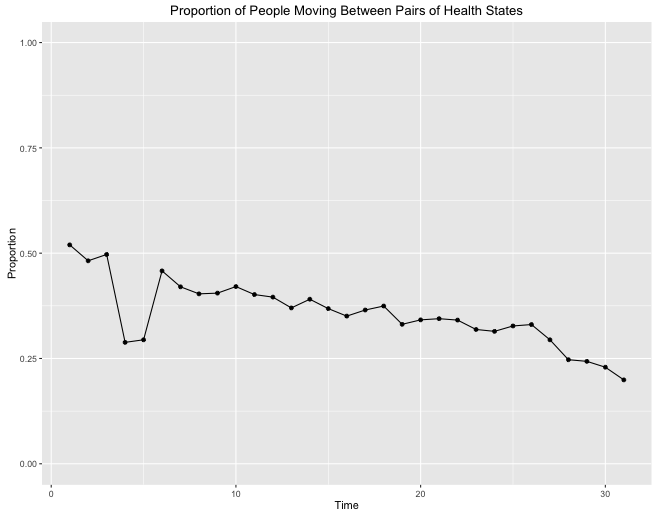
\includegraphics[scale=0.5]{Rplotp4p1}
			\end{figure}
			%b
			\item I chose to visualize this in a single graphic with counts on the vertical axis and time on the horizontal axis. I think  this plot is easy to visualize overall trends in the counts of people in different states as a function of time, but if we had several factors the graph could quickly become overwhelming and unable to interpret effectively, which it might even be at this point.
			\begin{figure}[H]
				\centering
				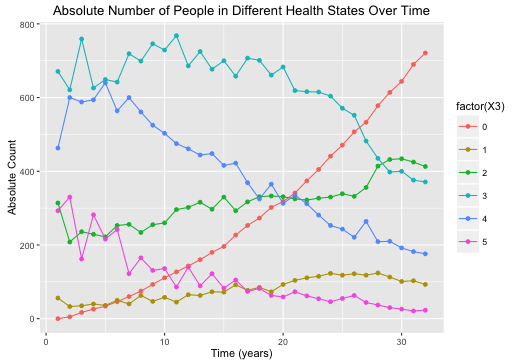
\includegraphics[scale=0.75]{Rplotp4p2}
			\end{figure}
			%c
			\item I chose to randomly sample 100 individuals from the data set and plot trajectories of all 100 individuals in a matrix using ggplot2. An obvious disadvantage is the fact that I sampled less than 10\% of the data set and it could be hard to detect overall average behavior. I think an advantage is that we can see a smaller representative rather than be overwhelmed by 1,797 plots of trajectories on a single figure.
			\begin{figure}[H]
			\caption{100 Trajectories of Patient Health over 32 Years}
				\centering
				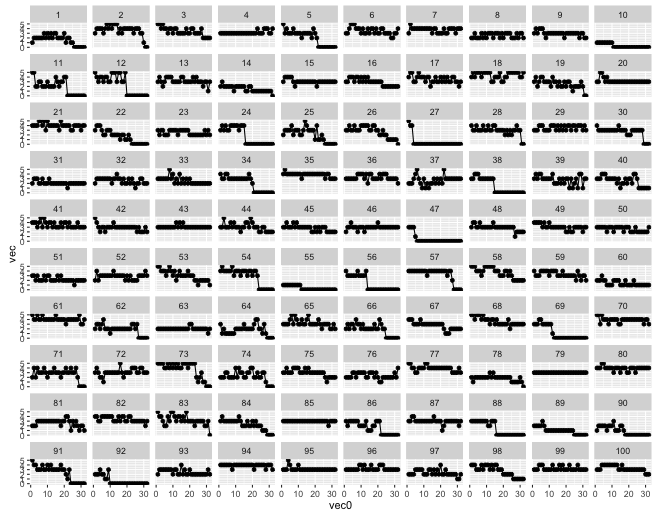
\includegraphics[scale=0.5]{Rplotp4p3}
			\end{figure}
		\end{enumerate}
\end{enumerate}
\newpage
Code for HW1
\begin{verbatim}
	library(sandwich)
setwd("~/Dropbox/UW2015-2016/Win2016/571/hw1")
##
##problem 1
##
dat1 <- read.table("rats.csv", header=TRUE, sep=',')
attach(dat1)
m1 <- glm(y~x, family=Gamma(link="log")) 
#we have a log link log(1/lambda_i) = beta_0 + beta_1x_i
sand <- vcovHC(m1,type="HC0")
beta <- m1$coefficients
n = length(x)
X = cbind(rep(1,n),x)
temp = exp(X%*%(-beta))
A = (-1/n)*matrix(c(y%*%temp, (x*y)%*%temp, (x*y)%*%temp, sum(x^2*y*temp)
  ), nrow=2, ncol=2
)

fun <- function(x,y)
{
  return(
    matrix(c(
      -1+y*exp(-beta[1]-x*beta[2]), -x+x*y*exp(-beta[1]-x*beta[2])
    ))
  )
}

B = matrix(0,nrow=2,ncol=2)
for(i in 1:n)
{
  B = B + fun(x[i],y[i])%*%t(fun(x[i],y[i]))
}
B = B/n

yum = solve(A)%*%B%*%solve(A)/n
yum2 = solve(Ah)%*%B%*%solve(Ah)/n
detach(dat1)

##
##problem 3
##
library(MASS)
n = dim(cars)[1]
R <- function(rho)
{
  temp = matrix(0, nrow=n, ncol=n)
  for(i in 1:n)
  {
    for(j in 1:n)
    {
      temp[i,j] = rho^(abs(i-j))
    }
  }
  return(temp)
}

#|rho| < 1 for full column rank
X = cbind(rep(1,n), cars$dist)
probs <- function(sigmasq,rho){
  countint = 0
  countslope = 0
  for(i in 1:10000)
  {
    y = X%*%beta + mvrnorm(1,rep(0,n),sigmasq*R(rho))
    m1 <- lm(y~cars$dist)
    temp = confint.default(m1)
    if(
      findInterval(beta[1], temp[1,])==1 #is beta1 in the 95% interval?
      )
    {
      countint = countint + 1
    }
    if(
      findInterval(beta[2], temp[2,])==1 #is beta2 in the 95% interval?
    )
    {
      countslope = countslope + 1
    }
  }
  return(c(countint/10000
  ,countslope/10000))
}

set.seed(1)
sigmas <- c(0.1,1,10,100)
rhos <- c(-0.9,-0.5,-0.25,0,0.25,0.5,0.9)
beta = c(1,-1)
for(sig in sigmas){
  for(rho in rhos)
  {
    cat("coverage for ", sig, rho, probs(sig,rho),"\n")
  }
}  

beta = c(5,30)
for(sig in sigmas){
  for(rho in rhos)
  {
    cat("coverage for ", sig, rho, probs(sig,rho),"\n")
  }
}  


probs(1,0.5)


H = X%*%solve(t(X)%*%X)%*%t(X)
sum(diag((diag(n)-H)%*%R(0.9))) #

##
##p4
##
p4 <- read.table("evggfpd30.csv", header=TRUE, sep=",")
library(ggplot2)
m <- dim(p4)[1] #this many people
n <- dim(p4)[2]

prop = rep(0,n-1)
for(i in 1:31)
{
  prop[i] = m - sum(p4[,i]==p4[,i+1])
}

prop = prop / m
dftemp = data.frame(cbind(1:31,prop))
plotp1 <- ggplot(dftemp, aes(x=V1, y=prop))
plotp1 + geom_point() + geom_line() + ylim(c(0,1)) + xlab("Time") 
+ ylab("Proportion") + ggtitle("Proportion of People Moving Between Pairs of Health States")

##p4p2

countsPerYear <- apply(p4,2,table) #compute counts of levels per year

zeros = as.matrix(p4) == matrix(0,nrow=m,ncol=n)
ones = as.matrix(p4) == matrix(1,nrow=m,ncol=n)
twos = as.matrix(p4) == matrix(2,nrow=m,ncol=n)
threes = as.matrix(p4) == matrix(3,nrow=m,ncol=n)
fours = as.matrix(p4) == matrix(4,nrow=m,ncol=n)
fives = as.matrix(p4) == matrix(5,nrow=m,ncol=n)
dead = cbind(unname(apply(zeros,2,sum)),rep(0,32))
poor = cbind(unname(apply(ones,2,sum)),rep(1,32))
fair = cbind(unname(apply(twos,2,sum)),rep(2,32))
good = cbind(unname(apply(threes,2,sum)),rep(3,32))
vgood = cbind(unname(apply(fours,2,sum)),rep(4,32))
eggs = cbind(unname(apply(fives,2,sum)),rep(5,32))


p4p2 <- data.frame(cbind(rep(1:32,6),rbind(dead, poor, fair, good, vgood, eggs)), row.names=NULL)
plot <- ggplot(p4p2, aes(X1, X2, color=factor(X3))) + geom_point() + geom_line() 
+ xlab("Time (years)") + ylab("Absolute Count")
plot <- plot + ggtitle("Absolute Number of People in Different Health States Over Time")


##p4p3
set.seed(1)
people <- sample(seq(1,m), 100, replace=TRUE)
temp = as.matrix(p4[people,])
vec = c()
vec2 = c()
for(i in 1:100)
{
  vec = append(vec,temp[i,])
  vec2 = append(vec2, rep(i,32))
}
vec0 = rep(1:32,100)
df <- data.frame(cbind(vec0,vec,vec2), row.names=NULL)


ggplot(df, aes(vec0,vec)) + geom_point() + geom_line() + facet_wrap(~vec2)
\end{verbatim}
\end{document}



